\section{부록}

$\pi$ 라디안은 180도. 1라디안은 $180 \over \pi$도. 1도는 $\pi \over 180$ 라디안. 아래 그림은 각도, 라디안, $\cos$, $\sin$ 순서.

\begin{figure}[h]
  \centering
  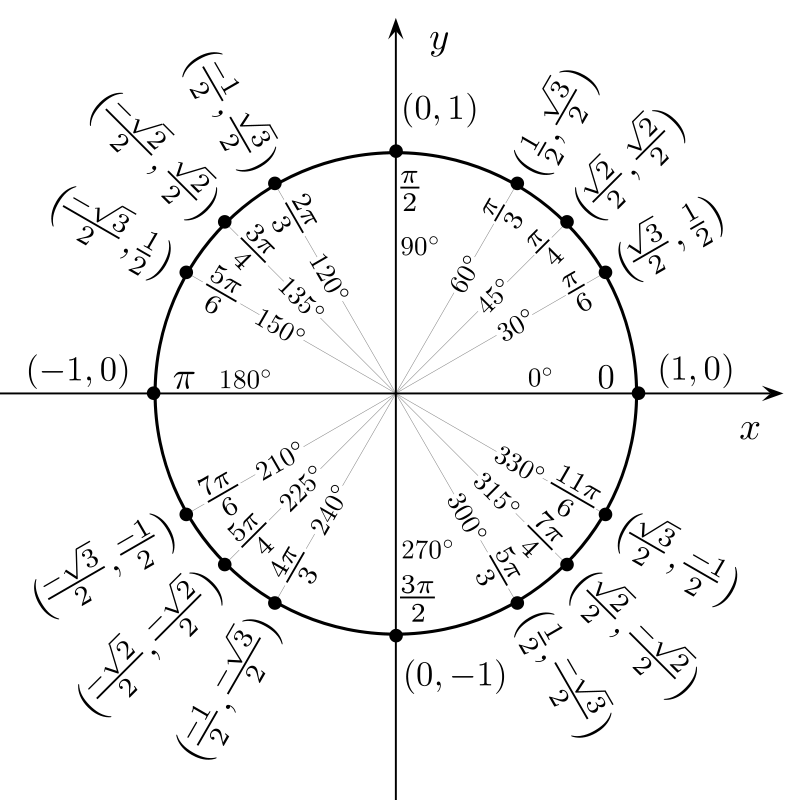
\includegraphics[width=\columnwidth]{unit-circle-angles.png}
\end{figure}

반시계 방향으로 $\theta$는 시계 방향으로 $-\theta$, 이때: $\sin{-\theta} = -\sin{\theta}$, $\cos{-\theta} = \cos{\theta}$

\begin{figure}[h]
  \centering
  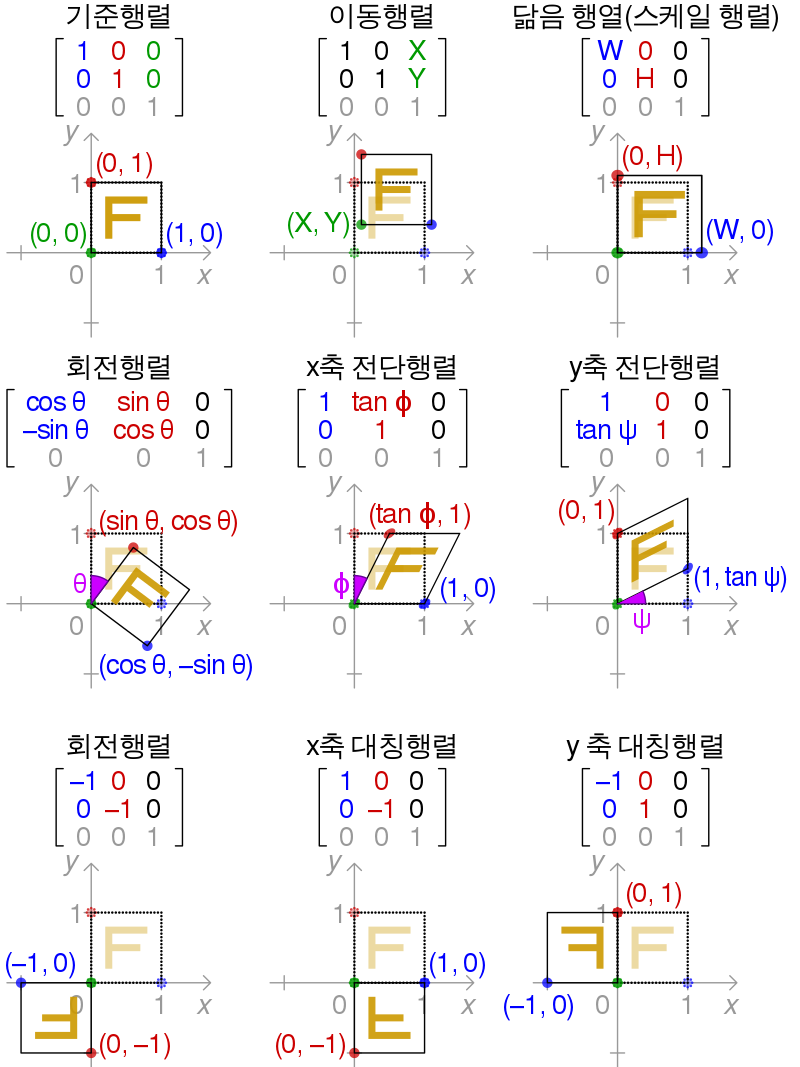
\includegraphics[width=\columnwidth]{transformation-matrix.png}
\end{figure}

\begin{verbatim}
mat3 getTBN(vec3 N) {
  vec3 Q1 = dFdx(worldPosition);
  vec3 Q2 = dFdy(worldPosition);
  vec2 st1 = dFdx(texCoords);
  vec2 st2 = dFdy(texCoords);
  float D = st1.s * st2.t - st2.s * st1.t;
  return mat3(
    normalize((Q1 * st2.t - Q2 * st1.t) * D),
    normalize((-Q1 * st2.s + Q2 * st1.s) * D),
    N,
  );
}

void main(void) {
  vec3 l = lightPosition - worldPosition;
  vec3 L = normalize(l);
  vec3 N = normalize(normal);

  mat3 tbn = getTBN(N);
  float dBdu = texture(
    bumpTex, texCoords + vec2(0.00001, 0)
  ).r - texture(bumpTex,
                texCoords - vec2(0.00001, 0)).r;
  float dBdv = texture(
    bumpTex, texCoords + vec2(0, 0.00001)
  ).r - texture(bumpTex,
                texCoords - vec2(0, 0.00001)).r;
  N = normalize(N - dBdu * tbn[0] * 100 -
    dBdv * tbn[1] * 100);

  vec3 V = normalize(cameraPosition -
                     worldPosition);
  vec3 R = 2 * dot(L, N) * N - L;
  vec3 I = lightColor / dot(l, l);
  vec4 diffColor = texture(diffTex, texCoords);
  vec3 c = diffColor.rgb * max(0, dot(L, N)) *
           I + diffColor.rgb * ambientLight;
  c += pow(max(0, dot(R, V)), shininess) * I;

  out_Color = vec4(pow(c, vec3(1 / 2.2)), 1);
}
\end{verbatim}
